\section{Sampling the MDM in the discrete and the continuum}
If we forget about the directions of the edges in $\vec{G}_n(\nu)$, the resulting undirected graph is supercritical, and, with high probability, the graph contains a unique giant component with surplus going to infinity as $n\to \infty$ (see e.g. \cite{molloyCriticalPointRandom1995,molloySizeGiantComponent1998,jansonNewApproachGiant2009} for a discussion of the phase transition in the undirected configuration model). This suggests that if we do not dismiss a large amount of edges, we will not be able to study the digraph in enough detail to find a metric space scaling limit of the SCCs. Therefore, we will not try to sample the entire digraph, but focus on the information that we need to find the SCCs. We start by studying the discrete digraph model, with the goal of identifying which edges can be part of an SCC, and how to sample them. In Subsection \ref{subsubsec.defcandidates}, we establish necessary conditions for an edge to be part of an SCC. These conditions imply that we only need to study the out-forest, and the surplus edges corresponding to a small subset of the dummy leaves. We call these dummy leaves \emph{candidates}. In Subsections \ref{subsubsec.samplingoutforest} and \ref{subsubsec.samplecandidates} we study the law of the out-forest and the surplus edges corresponding to the candidates respectively, and we define a procedure to sample them both. This yields a sequence of directed multigraphs with edge lengths in which the SCCs are embedded.  
In Subsection \ref{subsec.limitobject}, we define the continuous counterpart of the sampling procedure. The resulting object will be the limit under rescaling of the sequence of directed multigraphs with edge lengths in which the SCCs are embedded that was constructed in Subsections \ref{subsubsec.samplingoutforest} and \ref{subsubsec.samplecandidates}. 
\subsection{The discrete case}\label{subsec.discrete}
We will discuss the different type of edges that we can encounter in the exploration. Recall from Subsection \ref{sec:proofoutline} that by slight abuse of terminology, we call the dummy leaf that corresponds to a surplus edge its tail.

\subsubsection{Necessary conditions for an edge to be part of an SCC}\label{subsubsec.defcandidates}
Amongst the surplus edges, \emph{ancestral surplus edges}, which are surplus edges that point from a vertex to one of its ancestors, play a special role. All other surplus edges are called \emph{non-ancestral}. This is illustrated in Figure \ref{subfigure.typesofsurplusedges}. In Figure \ref{subfigure.sccinexample} we show how surplus edges affect the structure of the SCCs. This is the content of the next lemma.

\begin{figure}
\centering
\begin{subfigure}{0.8\textwidth}
 \centering
    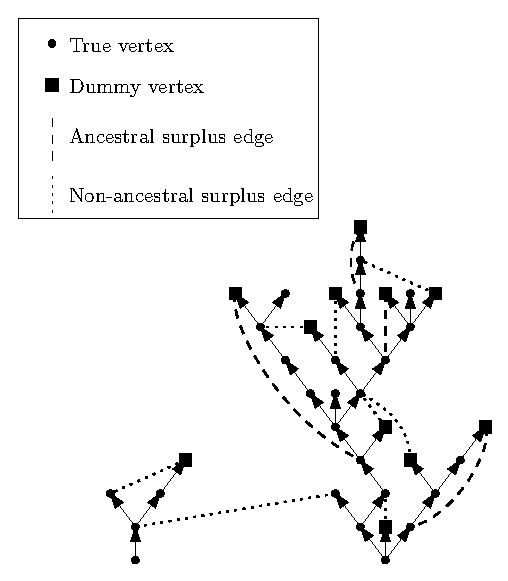
\includegraphics[scale=1.2]{Content/Pictures/Fig7a.eps}
    \caption{This figure illustrates an example of a depth-first exploration of two out-components with the different type of surplus edges highlighted. The ancestral surplus edges point from a vertex $v$ to one of its ancestors. They are always part of an SCC.}
    \label{subfigure.typesofsurplusedges} 
\end{subfigure}\\
\begin{subfigure}{0.8\textwidth}
  \centering
  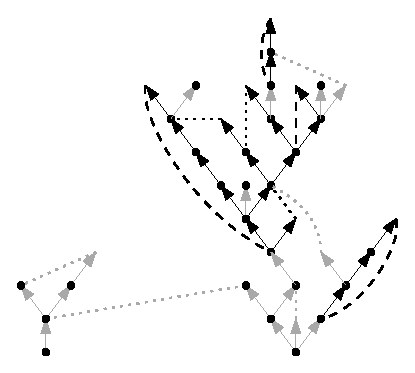
\includegraphics[scale=1.2]{Content/Pictures/Fig7b.eps}
  \caption{The edges that are part of an SCC are depicted in black. Two vertices are in the same SCC if and only if they are connected by black edges. }
    \label{subfigure.sccinexample}
\end{subfigure}
\caption{We illustrate the different types of surplus edges and how they affect the structure of the SCCs.}
\end{figure}

\begin{lemma}\label{lem:whatispartofscc}
The following facts hold for SCCs. 
\begin{enumerate}
\item \label{item.factsonsccs1}The vertices of an SCC are contained in precisely one of the components of the out-forest. 
\item \label{item.factsonsccs2} Ancestral surplus edges are always part of an SCC.
\item \label{item.factsonsccs4} A non-ancestral surplus edge is part of an SCC only if its head is an ancestor of the tail of a surplus edge that is part of an SCC.
\item \label{item.factsonsccs4andabit} An edge in the out-forest is part of an SCC only if its head is an ancestor of the tail of a surplus edge that is part of an SCC.
\item \label{item.factsonsccs5} For any non-trivial SCC, the first surplus edge of the SCC that is explored is an ancestral surplus edge, and a component of the out-forest contains an SCC if and only if it contains an ancestral surplus edge.
\end{enumerate}
\end{lemma}
\begin{proof}
We start with \ref{item.factsonsccs1}. Let $v$ and $w$ be two vertices in the same SCC. Without loss of generality, $v$ is explored first in depth-first order in the out-direction. Since $v$ and $w$ are part of the same SCC, we know that there is a path from $v$ to $w$ in the out-direction. This implies that $w$ will be part of the out-subtree consisting of the descendants of $v$. This implies that they are part of the same component of the out-forest.

To prove \ref{item.factsonsccs2}, suppose there is an ancestral surplus edge from $v$ to $w$. This implies that $w$ is an ancestor of $v$ in an out-component, which implies that there is a path from $w$ to $v$ as well. It follows that $w$ and $v$ are in the same SCC and that the ancestral surplus edge from $v$ to $w$ is in this SCC as well. 

To prove \ref{item.factsonsccs4} and \ref{item.factsonsccs4andabit}, suppose there is a non-ancestral surplus edge from $v$ to $w$ that is part of an SCC, or that $(v,w)$ is an edge in the out-forest that is part of an SCC. Then, there is some directed path $(x_0,\dots, x_m)$ with $x_0=w$ and $x_m=v$. Let $k$ be minimal such that $x_k$ is not a descendant of $w$ (such a $k$ exists, because by assumption, $v$ is not a descendant of $w$). Then, $(x_{k-1},x_k)$ is a surplus edge that is in the same SCC as $v$ and $w$, and $x_{k-1}$ is a descendant of $w$ by definition of $k$.


Finally, \ref{item.factsonsccs2} and \ref{item.factsonsccs4} imply \ref{item.factsonsccs5}. 
\end{proof}
 \cref{lem:whatispartofscc} motivates the following definition.
\begin{definition}\label{def.candidate}
A dummy vertex is a \emph{candidate} if one of the following statements holds for the surplus edge that it corresponds to. 
\begin{itemize}
    \item It is an ancestral surplus edge, or
    \item Its head is the ancestor of a candidate.
\end{itemize}
\end{definition}
The following proposition is at the core of our strategy to study the SCCs.
\begin{proposition}\label{prop:edgesinSCCs}
Any edge that is part of an SCC is either a surplus edge corresponding to a candidate, or is contained in the subforest of the out-forest that is spanned by the candidates and the roots of the out-components.
\end{proposition}
\begin{proof}
This follows from Definition \ref{def.candidate} and \cref{lem:whatispartofscc}.
\end{proof}

\cref{prop:edgesinSCCs} implies that to sample the SCCs, we do not need to sample the heads corresponding to all dummy leaves. Instead, for every dummy leaf, we only need to know whether it is a candidate, and if so, where its head is. 
\subsubsection{Sampling the out-forest}\label{subsubsec.samplingoutforest}
This subsection discusses how to obtain the out-forest conditional on the order in which the vertices are discovered. We will study the law of the degrees in order of discovery in \cref{sec:measure-change}. The out-forest is obtained in the following way. Let $(\mathbf{\hat{D}}_{n,1},\dots,\mathbf{\hat{D}}_{n,n})$ be the degree pairs in order of discovery (i.e. the order given by $\exploredvertices$ in Algorithm \ref{alg:edfs}). Up to time-step $k$, suppose we have discovered the first $m\leq k<n$ elements of  $(\mathbf{\hat{D}}_{n,1},\dots,\mathbf{\hat{D}}_{n,n})$. Then, at time $k+1$,
\begin{enumerate}
    \item If we have finished a component of the out-forest, let the next out-component have a root with out-degree $\hat{D}_{n,m+1}^+$. 
    \item Otherwise,
    \begin{enumerate}\item With probability proportional to the total in-degree of the undiscovered vertices, i.e. $\sum_{i={m+1}}^{n} \hat{D}_{n,i}^-$, let the next vertex in depth-first order be a true vertex with out-degree $\hat{D}_{n,m+1}^+$. 
    \item With probability proportional to the number of unpaired in-half-edges of the $m$ discovered vertices, let the next vertex in depth-first order be a dummy leaf, and reduce the total number of unpaired in-edges of the $m$ discovered vertices by $1$.
\end{enumerate}
\end{enumerate}
We make this rigorous in the following proposition.
\begin{proposition}\label{prop:sampleoutforest}
Suppose that the sequence of degrees in order of discovery $(\mathbf{\hat{D}}_{n,1},\dots,\mathbf{\hat{D}}_{n, n})$ is given. Suppose that after time-step $k$, there are still unpaired out-half-edges. Suppose that for $1\leq l\leq k$, that up to time $l$, $\hat{P}_n(l)$ surplus edges have been sampled. Then, $$\left(\hat{S}^+_n(l),1\leq l\leq k \right):=\left(\sum_{i=1}^{l-\hat{P}_n(l)}\hat{D}^+_{n,i}-l,1\leq l\leq k\right)$$ is the \L ukasiewicz path of the out-forest up to time $k$. Moreover, for $$\left(\hat{I}^+_n(l),1\leq l\leq k\right):=\left(\min\left\{\hat{S}^+_n(m):1\leq m \leq l\right\},1\leq l \leq k \right),$$
define 
$$\left(\hat{S}^-_n(l),1\leq l \leq k\right):=\left(\sum_{i=1}^{l-\hat{P}_n(l)}\hat{D}^-_{n,i}-l-\hat{I}^+_n(l)+1,1\leq l\leq k\right),$$
so that $\hat{S}^-_n(k)$ is equal to the number of unpaired in-half-edges of discovered vertices at time $k$. Then, the probability that we sample a surplus edge at the $(k+1)$th time-step is given by
$$\frac{\hat{S}^-_n(k+1)}{\sum_{i=1}^n D^-_i-k-\hat{I}^+_n(k)+1}\one_{\left\{\hat{I}^+_n(k)=\hat{I}^+_n(k-1)\right\}}.$$
We do not need to know the position of the heads of the surplus edges in order to sample the out-forest.
\end{proposition}
\begin{proof}
Note that if up to time $k$, $\hat{P}_n(k)$ surplus edges have been sampled, this implies that $k-\hat{P}_n(k)$ true vertices have been discovered. Thus, up to time $k$, the out-forest contains $\hat{P}_n(k)$ dummy leaves, and true vertices with degrees $(\hat{D}^+_{n,1},\dots,\hat{D}^+_{n,k-\hat{P}_n(k)})$, so by definition of the \L ukasiewicz path, its value is indeed equal to $\hat{S}^+_n(k)$ at time $k$. Moreover, up to time $k$, the total in-degree of the discovered true vertices is equal to $\sum_{i=1}^{k-\hat{P}_n(k)}\hat{D}^-_{n,i}$. At every time-step, we pair one in-half-edge of a discovered vertex, unless we start a new component. The value $-\hat{I}^+_n(k)$ corresponds to the number of out-components that are fully explored up to time $k$, so the total number of unpaired in-half-edges of discovered vertices at time $k$ is equal to $\hat{S}^-_n(k)$. By the same reasoning, the total number of unpaired in-half-edges is equal to $\sum_{i=1}^n D^-_i-k-\hat{I}^+_n(k)+1$. The probability of sampling a surplus edge at step $(k+1)$ follows. We note that this probability does not depend on the positions of the heads of the surplus edges, but only on their number, which implies that we can sample the out-forest without sampling the positions of the heads.
\end{proof}
\subsubsection{Sampling the candidates}\label{subsubsec.samplecandidates}
We will now study the law of the candidates and their heads conditional on the out-forest. We will first identify the candidates amongst the dummy leaves, and then we will sample the positions of their heads. 


If the vertex discovered at time $k$ is a dummy leaf, the head of the corresponding surplus edge is a uniform pick from the $\hat{S}^-(k)$ unpaired in-half-edges of discovered vertices at time $k$. Therefore, the probability that a dummy leaf added at time $k$ corresponds to an ancestral surplus edge is given by the number of unpaired in-edges on its path to the root divided by $\hat{S}^-(k)$. This implies that to understand the law of the position of ancestral surplus edges, we need to understand where the unpaired in-edges are. 


We will study this by modifying the edge lengths in the out-forest. We extend our definitions in \cref{sec:proofoutline} to trees with edge lengths as follows. Suppose $T=(V,E,\rho)$ is an ordered rooted finite tree, and suppose we have a function $\ell:E\to [0,\infty)$. Then, we can view $T$ as a metric space by regarding an $e$ as a line segment with length $\ell(e)$. The distance $d^\ell_T$ between points $a_1$ and $a_2$ on line segments $l_1$ and $l_2$ respectively is then defined as the length of the unique non-self-intersecting path between $a_1$ and $a_2$ that traverses the line segments of the tree, and we denote the resulting metric space $(T,d^\ell_T)$ by $\mathrm{T}^\ell$, and call it a \emph{ordered rooted finite tree with edge lengths}. This gives rise to an alternative height process, referred to as $h^\ell$, which is defined $$h^\ell(i)=d^\ell_T(v_i,v_0),$$ i.e.  for all $i$, $h^\ell(i)$ equals the distance from $v_i$ to the root in $\mathrm{T}^\ell$. We set the \L ukasiewicz path of $\mathrm{T}^\ell$ equal to the \L ukasiewicz path of $\mathrm{T}$.

We will now study the positions of the unpaired in-edges by modifying the edge lengths as follows: for a vertex $v$ with in-degree $m$, the edges connecting it to its children will all have length $m-1$ (unless $v$ is the root of an out-component, in which case the edges connecting to its children will be assigned length $m$). The height of vertex $w$ in this forest with modified edge lengths corresponds to the number of in-half-edges that can be used to form an ancestral surplus edge with tail $w$. We assign lengths to all edges in the out-forest and call the resulting forest with edge lengths \emph{the out-forest with edge lengths}. Denote the height process of the out-forest with edge lengths by $(\hat{H}_n^\ell(k),k\geq 1)$. 
Recall from Lemma \ref{lem:whatispartofscc} that the surplus edge corresponding to the first candidate in any component of the out-forest is ancestral. The following proposition illustrates the importance of $\hat{H}^\ell$ in finding the first ancestral surplus edges in the out-components.

\begin{proposition}\label{prop:probancestral}
Consider the exploration of the out-forest at time $k$. If no ancestral surplus edge has been sampled in the current component, then the probability that the $k$th vertex in depth-first order is a candidate is given by 
$$\frac{\hat{H}^\ell(k)}{\hat{S}_n^-(k)}\one_{\{\hat{P}_n(k)-\hat{P}_n(k-1)=1\}}.$$
This event is conditionally independent of the positions of the heads of the surplus edges that were found before time $k$, given that none of them were ancestral in the current component.
% If $k$ is the tail of an ancestral surplus edge, then the position of the end point $Y$ has the following law. Let $U$ be uniform on $[0,\hat{H}^\ell(k)]$. Then, let $Y_k$ be the height of youngest ancestor $l$ of $k$ such that $H^{\ell}(l)<U$. 
\end{proposition}
\begin{proof}
We claim that if no ancestral surplus edge has been sampled in the current component, none of the ancestors of $k$ are the head of a surplus edge. Indeed, for $x$ an ancestor of $k$, all vertices that are discovered since the discovery of $x$ up to time $k$ are descendants of $x$, because the out-forest is explored in a depth-first manner. Therefore, any surplus edge with head $x$ sampled up to time $k$ is ancestral. This implies that for $d^-$ the in-degree of $x$, the number of unpaired in-half-edges of $x$ at time $k$ is equal to $d^--1$ (unless $x$ is the root of the out-component, in which case it has $d^-$ unpaired in-half-edges).

Therefore, the number of unpaired in-half-edges corresponding to ancestors of $k$ is equal to $H^\ell(k)$. Moreover, note that, by definition of the dummy leaves, $k$ is the tail of a surplus edge if and only if $k$ is a dummy leaf, i.e. if and only if $\hat{P}_n(k)-\hat{P}_n(k-1)=1$. In that case, the probability that it connects to given unpaired in-half-edge of a discovered vertex is equal to $1/\hat{S}_n^-(k)$. The stated probability follows. The independence of the positions of the heads of earlier surplus edges is immediate.
\end{proof}

We now illustrate how to find the other candidates in a component of the out-forest. 

Let $T^n_{g_n}$ be a component of the out-forest with root $g_n+1$ and component size $\sigma_n$. Suppose the first ancestral surplus edge with vertices in $T^n_{g_n}$ corresponds to a dummy leaf $V^n_1\in [g_n+2,g_n+\sigma_n]$. Let $V^n_1<k\leq g_n+\sigma_n$, and suppose the candidates found up to time $k$ are given by $V^n_1,\dots,V^n_m$. Let $T^{n,\mathrm{mk}}_k$ be the subtree of $T^n_{g_n}$ spanned by $\{g_n+1,V^n_1,\dots,V^n_m,k\}$, and let $\ell(T^{n,\mathrm{mk}}_k)$ be its total length with edge lengths as encoded by $(\hat{H}^\ell(i),i\in [g_n+1,g_n+\sigma_n])$.
\begin{proposition}
\label{prop:samplecandidates}
 The probability that $k$ is a candidate is given by 
$$\frac{\ell\left(T^{n,\mathrm{mk}}_k\right)-m}{\hat{S}^-(k)}\one_{\{\hat{P}_n(k)-\hat{P}_n(k-1)=1\}}.$$
\end{proposition}
\begin{proof}
Note that if $k$ is a dummy leaf, it gets paired to a uniform pick from the $\hat{S}^-(k)$ as-yet unpaired in-half-edges of discovered vertices. By Definition \ref{def.candidate}, in that case, $k$ is a candidate if and only if the head of its corresponding surplus edge is in $T^{n,\mathrm{mk}}_k$. Observe that $\ell\left(T^{n,\mathrm{mk}}_k\right)$ is equal to the number of in-half-edges of $T_{k}$ that can be used to form surplus edges. By the definition of a candidate, exactly $m$ of those have been paired: one for each element in $\{V^n_1,\dots,V^n_m\}$. This implies that $\ell\left(T^{n,\mathrm{mk}}_k\right)-m$ of the $\hat{S}^-(k)$ options will cause $k$ to be a candidate.
\end{proof}

Note that the probability that a dummy leaf is a candidate only depends on the out-forest and the number of candidates that have been found in the component so far. The position of the heads of the surplus edges corresponding to candidates can be found as follows.

Let $T^n_{g_n}$ be a component of the out-forest with root $g_n+1$ and component size $\sigma_n$. Suppose its candidates are given by $\{V^n_1,\dots,V^n_{N_n}\}$. Then, for $1\leq i\leq {N_n}$, suppose the heads of the surplus edges corresponding to $V^n_1,\dots,V^n_{i-1}$ are given by $W_1^n,\dots,W^n_{i-1}$ respectively. 
\begin{proposition}
\label{prop.sampleheadcandidates}
The in-half-edge that $V^n_{i}$ gets paired to is a uniform pick from the $$\ell\left(T^{n,\mathrm{mk}}_{V^n_i}\right)-(i-1)$$ unpaired in-half-edges of $T^{n,\mathrm{mk}}_{V^n_i}$ that remain.
\end{proposition}
\begin{proof}
Given that $V^n_{i}$ is a candidate, its head will be in $T^{n,\mathrm{mk}}_{V^n_i}$. Then, the distribution follows.
\end{proof}

Propositions \ref{prop:sampleoutforest}, \ref{prop:probancestral}, \ref{prop:samplecandidates}, and \ref{prop.sampleheadcandidates} justify the following sampling procedure.
\begin{enumerate}
    \item Sample the out-forest, and suppose it has $N$ vertices.
    \item Define a counting process $(A_n(k),k\leq N)$, with the probability of an increment at time $k$ given by $$\frac{\hat{H}_n^\ell(k)}{\hat{S}_n^-(k)}\one_{\{\hat{P}_n(k)-\hat{P}_n(k-1)=1\}}.$$
    \item For $i\geq 1$, let $X_i^n=\min\{k:A_n(k)=i\}$ be the time that the $i$th ancestral surplus edge is sampled. For $i\geq 1$, let $G_i^n$ be the left endpoint of the excursion of $\hat{S}^{+}_n$ above its running infimum that encodes the out-component that contains the $i$th ancestral surplus edge, and let $\Sigma_i^n$ be the length of this excursion, i.e. 
\begin{align*}G_i^n&=\min\left\{k\geq 1:\hat{S}^{+}_n(k)=\min\{\hat{S}^{+}_n(l):l\leq X_i^n\}\right\}\\
\Sigma_i^n&=\min\left\{k \geq 1: \min\left\{\hat{S}^{+}_n(l):l\leq G_i^n+k\right\} < \min\left\{\hat{S}^{+}_n(l):l\leq X_i^n\right\}\right\},
\end{align*}
so that for each $i\geq 1$, the excursion $\left(\hat{S}^+(k),k\in [G_i^n+1,G_i^n+\Sigma_i^n]\right)$ encodes the out-tree containing $X_i^n$. For each $(g_n,\sigma_n)\in \{(G_i^n,\Sigma_i^n)\}$, let $T^n_{g_n}$ be the tree in out-forest with root $g_n+1$, and do the following.
    \begin{enumerate}
    \item \label{item.procedure3} Set $V_1^n=\min\{m\geq 1:A_n(m)=A_n(g_n)+1\}$, and find the other candidates $\{V_2^n,\dots ,V_{N_n}^n\}$ according to the procedure described in the statement of \cref{prop:samplecandidates}.
    \item \label{item.procedure4} For the tails $V_1^n,\dots, V_{N_n}^n$, sample their corresponding heads $W_1^n,\dots ,W_{N_n}^n$ respectively according to the procedure described in the statement of \cref{prop:samplecandidates}.
    \item Let $T^{n,\mathrm{mk}}(g_n)$ be the subtree of $T^n_{g_n}$ spanned by $\{g_n+1,V_1^n,\dots ,V_{N_n}^n\}$. Then, quotient it by the equivalence relation $\sim$ which identifies $V_i^n$ and $W_i^n$ for each $1\leq i\leq N_n$ to obtain a rooted metric space with surplus $N_n$ $$M^n_{g_n}=T^{n,\mathrm{mk}}(g_n)/\sim.$$ 
\end{enumerate}
\end{enumerate}
Then, all SCCs of $\vec{G}_n(\nu)$ are sub-digraphs of $\left\{M^n_{G_i^n}, i\geq 1 \right\}$. Call the kernels of these SCCs, ordered by decreasing size, $(C_i(n),i\geq 1)$, completed with an infinite repeat of $\mathfrak{L}$. Observe that we may view $M^n_{G_i^n}$ as a finite rooted directed multigraph $M^n_{G_i^n}$ whose edges are endowed with lengths. To be precise, in  $M^n_{G_i^n}$, let the vertex set consist of $G_i^n+1$, $W_i^n$ for $i\leq N_n$, and the branch points $V_i^n\wedge V_j^n$ for $i\neq j\leq N_n$. Then, we obtain $(C_i(n),i\geq 1)$ by ordering the kernels of the non-trivial SCCs in $\left\{M^n_{G_i^n}, i\geq 1 \right\}$ by decreasing size, and completing the list with an infinite repeat of $\mathfrak{L}$. See Figures \ref{figure.extractSCCs1}, \ref{figure.extractSCCs2} and \ref{figure.extractSCCs3} for an illustration of this procedure.

\begin{figure}
\centering
\begin{subfigure}{.7\textwidth}
 \centering
    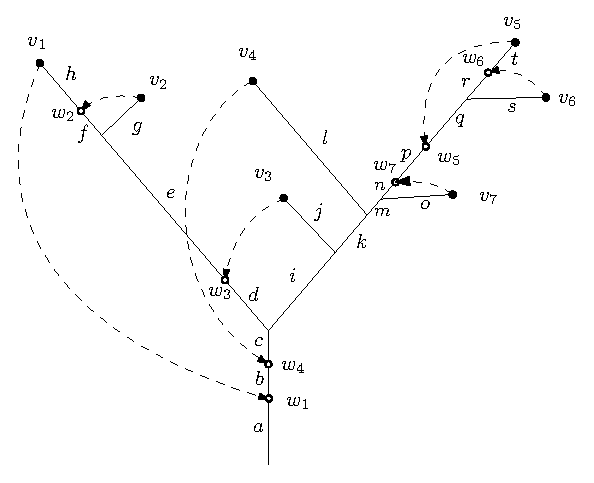
\includegraphics[width=0.8\linewidth]{Content/Pictures/out_componentswithmarks.eps}
    \caption{This is a subtree of an out-component spanned by the root of the out-component and the candidates $(v_1,\dots,v_7)$. Call the marked tree $T^{\mathrm{mk}}$. The heads of the surplus edges corresponding to candidates are denoted by $(w_1,\dots,w_7)$. }
\label{figure.extractSCCs1}
\end{subfigure}\\
\vspace{1.5em}
\begin{subfigure}{.8\textwidth}
  \centering
  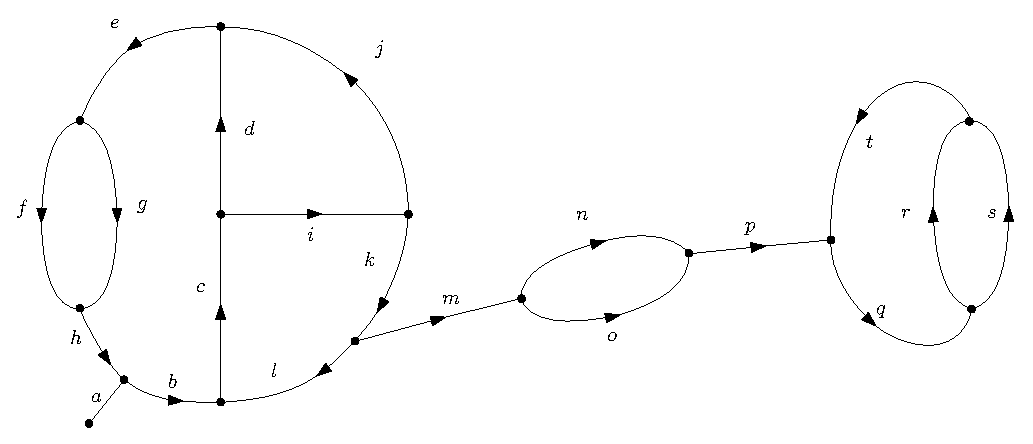
\includegraphics[width=0.9\linewidth]{Content/Pictures/Fig8a.eps}
  \caption{Identifying $v_i$ with $w_i$ for $i\in [7]$ gives $M$.}
  \label{figure.extractSCCs2}
\end{subfigure}\\
\vspace{1.5em}
\begin{subfigure}{.8\textwidth}
  \centering
  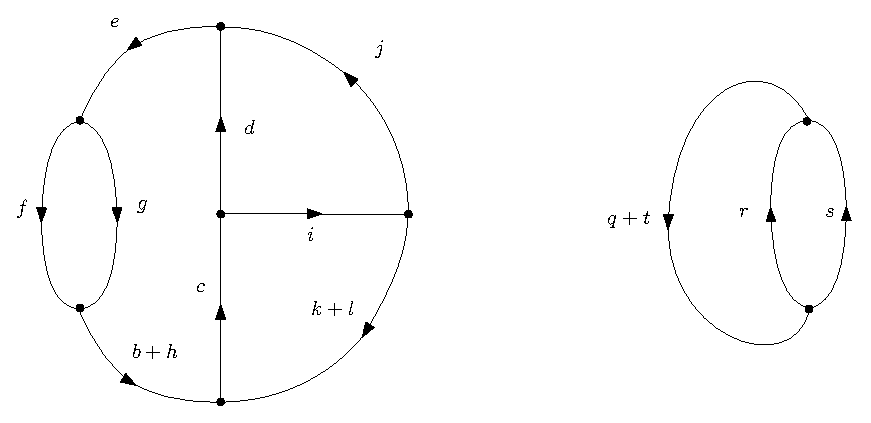
\includegraphics[width=0.9\linewidth]{Content/Pictures/Fig8b.eps}
  \caption{We find the SCCs that are contained in $M$.}
  \label{figure.extractSCCs3}
\end{subfigure}

\caption{We illustrate the procedure to find the SCCs in a component of the out-forest after finding the candidates. Taken from \cite{goldschmidtScalingLimitCritical2019} with permission of the authors.}
\end{figure}

\subsection{The continuum case}\label{subsec.limitobject}

We will define now define the continuous counterpart of the sampling procedure of the out-forest and the candidates. This is a modification of the procedure defined in Subsection 3.2.2 of \cite{goldschmidtScalingLimitCritical2019}.

\subsubsection{\texorpdfstring{$\R$}{R}-trees and their encoding}
The continuum analogue of discrete trees are given by $\R$-trees. We give the basic definitions here and refer the reader to the survey paper \cite{legallRandomTreesApplications2005} for more details. An $\R$-tree is a compact metric space $(\cT, d)$ such that for every $a, b \in \cT$ the following two properties hold:
\begin{enumerate}
    \item There exists a unique isometry $$i_{a, b} : [0, d(a, b)] \to \cT$$ such that $i_{a, b}(0) = a$ and $i_{a, b}(d(a, b)) = b$.
    \item If $q: [0, 1] \to \cT$ is any continuous map such that $q(0) = a$ and $q(1) = b$ then the image of $q$ is the same as the image of $i_{a, b}$.
\end{enumerate}
Let $\pathbtw{a, b}$ denote the image of $i_{a, b}$. This is the unique path between $a$ and $b$.

$\R$-trees are often encoded by continuous excursions which can be seen as a continuous analogue of the height function of a tree. Let $f: [0, \sigma] \to [0, \infty)$ be a continuous excursion, meaning $f$ is continuous, $f(0) = f(\sigma) = 0$ and $f(x) > 0$ for all $x \in (0, \sigma)$. Using $f$ we can define a pseudo-metric
\begin{equation*}
    d_f(x, y) = f(x) + f(y) - 2 \min_{s \in [x \wedge y, x \vee y]} f(s).
\end{equation*}
Using this we can define the quotient space
\begin{equation*}
    \cT_f = [0, \sigma] / \{d_f = 0\}.
\end{equation*}
The space $\cT_f$ equipped with the metric $d_f$ is the \emph{$\R$-tree encoded by the excursion $f$}. Let $p_f: [0, \sigma] \to \cT_f$ be the natural projection function. Then $\cT_f$ inherits a distinguished root vertex $\rho = p(0) = p(\sigma)$.

\subsubsection{The limit object}\label{subsubsec.samplecontinuousobject}
Let $(B_t,t\geq 0)$ be a standard Brownian motion, and set $$\left(\hat{B}_t,t\geq 0\right)=\left(B_t-\frac{\sigma_{-+}+\nu_-}{2\sigma_+\mu}t^2,t\geq 0\right).$$ 
\begin{remark}
We note that the coefficient of the parabolic drift of $\hat{B}$ is negative. Indeed, by definition of $\sigma_{+-}$ and $\nu_-$, the sign of the parabolic drift is the same as the sign of $\mu-\E[(D^-)^2D^+]$, and we note that
$$\frac{\E[(D^-)^2D^+]}{\E[D^+]}-\left(\frac{\E[D^+D^-]}{\E[D^+]}\right)^2=\frac{\E[(D^-)^2D^+]}{\mu}-1$$
is the variance of $D^-$ under the law of $\mathbf{D}$ size-biased by $D^+$, which is positive. Hence $\E[D^+(D^-)^2]/\mu\geq 1$, and the claimed negativity follows. 

\end{remark}
Define the reflected process
$$(\hat{R}_t,t\geq 0)= \left(\hat{B}_t-\inf\left\{\hat{B}_s: s\leq t\right\},t\geq 0\right).$$
Then, it follows from the argument in Section \ref{sec.convoutforest} that $\left(\frac{2}{\sigma_+}\hat{R}_t,t\geq 0\right)$ is the height process corresponding to an $\R$-forest with \L ukasiewicz path $\left(\sigma_+\hat{B}_t,t\geq 0\right)$. Call this forest the out-$\R$-forest. \\
Conditionally on $\hat{R}$, let $(A_t,t\geq 0)$ be a Cox process of intensity $$\frac{2(\sigma_{-+}+\nu_-)}{\sigma_+\mu^2} \hat{R}_t$$ at time $t$. Then, for $i$ in $\left\{1,2, \dots \right\}$, set $X_i=\min\{t:A_t=i\}$. For $i$ in $\left\{1,2,\dots \right\}$, define
\begin{align*}
G_i&=\inf\left\{t\geq 0:\hat{B}_t=\inf\{\hat{B}_s:s\leq X_i\}\right\}\text{ and}\\
\Sigma_i&=\inf\left\{ t\geq 0: \inf\{\hat{B}_s:s\leq G_i+t\} < \inf\{\hat{B}_s:s\leq X_i\}\right\},
\end{align*}
so that for each $i$ in $\left\{1,2,\dots \right\}$, $\left(\frac{2}{\sigma_+}\hat{R}_t,t\in [G_i,G_i+\Sigma_i]\right)$ encodes the $\R$-tree in the out-$\R$-forest that contains $X_i$. For each element of $\{(G_i,\Sigma_i):i=1,2,\dots\}$ we will sample the candidates in the $\R$-tree. Fix $i$, and set $(g,\sigma)=(G_i,\Sigma_i)$. Let $V_1=\inf\{s>0:A(s)=A(g)+1\}$, so that $g\leq V_1\leq g+\sigma$ by definition of $(g,\sigma)$. Let $\cT_g$ be the $\R$-tree encoded by $\left(\frac{2}{\sigma_+}\hat{R}_t,t\in [g,g+\sigma]\right)$ and let $p_g:[g,g+\sigma]\to \cT_l$ be the projection onto $\cT_g$ given by the encoding. Set $$||\cT_g||=\sup\left\{\frac{2}{\sigma_+}\hat{R}_t,t\in [g,g+\sigma]\right\},$$
the \emph{height} of $\cT_g$. \\
Suppose we have found candidates $\{V_1,\dots,V_m\}$. For $V_m\leq s\leq g+\sigma$, let $T^{\mathrm{mk}}_s$ be the subtree of $\cT_g$ spanned by $p_g\left(\{g,V_1,\dots,V_m,s\}\right)$, and let $|T^{\mathrm{mk}}_s|$ be its total length. Then, let $V_{m+1}$ be the first arrival time of a Poisson process on $[V_m,g+\sigma]$ of intensity $$\frac{\sigma_{-+}+\nu_-}{\mu^2}|T^{\mathrm{mk}}_s|ds.$$ If the process does not contain a point, let $\{V_1,\dots,V_m\}$ be the candidates of $\cT_g$, and set $N=m$. Otherwise, we repeat the inductive step for $\{V_1,\dots,V_{m+1}\}.$ If the induction does not terminate, we set $N=\infty$.\\
We show that $\P(N=\infty)=0$, by adapting the argument in Subsection 3.2.2 of \cite{goldschmidtScalingLimitCritical2019} to our set-up. Indeed, note that $V_m\leq s\leq V_{m+1}$ implies that  $|T^{\mathrm{mk}}_s|<(m+1)||\cT_g||$. Therefore, 
$$\P\left(\left.N\geq g+1,V_{m+1}-V_m<t \right|N\geq g\right)\leq \P(E_{m+1}<t),$$
for $(E_{k},k\geq 1)$ a sequence of exponential random variables with respective rates $$\frac{\sigma_{-+}+\nu_-}{\mu^2}k||\cT_g||.$$ 
Then,
$$\P\left(N=\infty \right)=\P\left(N=\infty\text{ and }\sup\{V_i:i\in \N\}<g+\sigma\right)\leq \P\left(\sum_{i=2}^\infty E_k\leq g+\sigma-V_1\right).$$
However, $\sum_{i=2}^\infty E_k=\infty$ a.s., because the harmonic series diverges, so, indeed, $\P\left(N<\infty \right)=1$. \\
Finally, for $1\leq i \leq N$, let the head corresponding to $V_i$, which we call $W_i$, be a uniform pick from the length measure on $T^{\mathrm{mk}}_{V_i}$. \\
Let $T^{\mathrm{mk}}(g)$ be the subtree of $\cT^{g}$ spanned by $\{g,V_1,\dots,V_N\}$. Then quotient $T^{\mathrm{mk}}(g)$ by the equivalence relation $\sim$ which identifies  $V_i$ and $W_i$ for each $1\leq i\leq N$ to obtain a rooted metric space $$\cM_{g}:=T^{\mathrm{mk}}(g)/\sim.$$ 
View $\cM_{g}$ as an element of $\vec{\cG}$ in the natural way. To be precise,  let the vertex set of $\cM_l$ consist of $g$, $W_i$ for $i\leq N$, and the branch points $V_i\wedge V_j$ for $i\neq j\leq N$. The directions are inherited from $\cT^l$, by considering all edges directed away from the root. Remove all edges that do not lie in an SCC of $\cM_{g}$ and delete any isolated vertices that are thus created. Then, apply the smoothing operation as defined in Subsection \ref{subsec.mdmkernels}. This creates a collection $\cC_g$ of strongly connected MDMs. Doing this for each $(g,\sigma)\in \{[G_i,\Sigma_i]\}$ yields the collection of strongly connected MDMs $\cC$ that has the law of the limit in Theorem \ref{thm.main}.

\subsubsection{Properties of the limit object}
We note that the limit object is encoded by $3$ parameters: the out-$\R$-forest is encoded by a Brownian motion with variance $\sigma_+^2$ and parabolic drift with coefficient $-(\sigma_{-+}+\nu_-)/(2\mu)$, and the identifications are a Cox process with intensity $(\sigma_{-+}+\nu_-)/\mu^2$ on the length measure of the subtree spanned by the previously found candidates and the currently explored vertex as described in Subsection \ref{subsubsec.samplecontinuousobject}. The limit object that is studied in \cite{goldschmidtScalingLimitCritical2019} corresponding to $\lambda=0$ (i.e. at criticality) is equal to our limit object in the case $\sigma_+^2=1$, $-(\sigma_{-+}+\nu_-)/(2\mu)=-1/2$, and $(\sigma_{-+}+\nu_-)/(\mu^2)=1$. Note that these three conditions are satisfied if we let $D^-$ and $D^-$ be independent $\operatorname{Poisson}(1)$ random variables. In \cite{goldschmidtScalingLimitCritical2019}, some properties of the limit object corresponding to these specific parameters are shown. A quick check shows that the proofs do not depend on the values of the parameters, so we deduce that the same properties also hold for our limit object. Let $\cM:=\bigcup_{G_i}\cM_{G_i}$.

\begin{proposition}
\begin{enumerate}
    \item The number of complex connected components of $\cM$ has finite expectation.
    \item The number of loops of $\cM$ is a.s. infinite.
\end{enumerate}
\end{proposition}

\begin{proposition}
\label{prop:allengthsaredifferent}
The SCCs of $\cM$ all have different lengths almost surely.
\end{proposition}
Write $\cC$ for the SCCs of $\cM$ and $\mathbf{C}_l$ for those of $\cM_l$, in decreasing order of length, with $\cM_l$ as defined in Subsection  \ref{subsubsec.samplecontinuousobject}. Write $\cC_{\text{cplx}}$ for the list of complex components of $\cC$ in decreasing order of length. For sequences $(K_1,\dots, K_j)$ and $(J_1,\dots,J_k)$ of directed multigraphs, write $(J_1,\dots,J_k)\equiv(K_1,\dots, K_j)$ if $j=k$ and $J_i$ is isomorphic to $K_i$ for each $i\leq j$. Extend this notation naturally to the case where one or both of the sequences has edge lengths by ignoring the edge lengths. 
\begin{theorem}
Let $K_1,\dots, K_j$ be a finite sequence consisting of $3$-regular strongly connected directed multigraphs or loops. We have 
$$\P\left[\cC_l\equiv(K_1,\dots, K_j)\right]>0.$$
Assuming that $K_1,\dots, K_j$ are all complex, we also have that 
$$\P\left[ \cC_{\text{cplx}}\equiv(K_1,\dots, K_j)\right]>0.$$
Let $(e_i,1\leq i \leq M)$ be an arbitrary ordering of the edges of $K_1,\dots, K_j$. Then, conditionally on $\cC_l\equiv(K_1,\dots, K_j)$, (resp. $\cC_{\text{cplx}}\equiv(K_1,\dots, K_j)$), $\cC_l$ (resp. $\cC_{\text{cplx}}$) gives lengths $(\ell(e_i),1\leq i \leq M)$ to these edges, and their joint distribution has full support in 
$$\left\{\mathbf{x}=(x_1,\dots, x_M)\in \R_+^M:\forall 1\leq i\leq j-1, \sum_{k:e_k\in E(K_i)}x_k \geq \sum_{k:e_k\in E(K_{i+1})}x_k\right\}.$$
\end{theorem}


